\documentclass[12pt,a4paper]{article}

% ── Encoding & language ──────────────────────────────────────────────────────
\usepackage[utf8]{inputenc}
\usepackage[T1]{fontenc}
\usepackage[italian]{babel}

% ── Layout ───────────────────────────────────────────────────────────────────
\usepackage[top=2.5cm, bottom=2.5cm, left=2.8cm, right=2.8cm]{geometry}
\usepackage{setspace}
\setstretch{1.05}

% ── Math ─────────────────────────────────────────────────────────────────────
\usepackage{amsmath, amssymb, amsthm}
\usepackage{bm}

% ── Graphics & color ─────────────────────────────────────────────────────────
\usepackage{graphicx}
\usepackage[table,xcdraw]{xcolor}
\usepackage{float}
\usepackage{subcaption}

% ── Code listings ────────────────────────────────────────────────────────────
\usepackage{listings}
\usepackage{inconsolata}

\definecolor{codebg}{RGB}{245,245,245}
\definecolor{codeframe}{RGB}{200,200,200}
\definecolor{kw}{RGB}{0,0,180}
\definecolor{str}{RGB}{163,21,21}
\definecolor{cmt}{RGB}{0,128,0}

\lstset{
  language=Python,
  backgroundcolor=\color{codebg},
  frame=single,
  rulecolor=\color{codeframe},
  basicstyle=\ttfamily\small,
  keywordstyle=\color{kw}\bfseries,
  stringstyle=\color{str},
  commentstyle=\color{cmt}\itshape,
  numbers=left,
  numberstyle=\tiny\color{gray},
  numbersep=8pt,
  breaklines=true,
  showstringspaces=false,
  tabsize=4,
  captionpos=b,
}

% ── Tables ───────────────────────────────────────────────────────────────────
\usepackage{booktabs}
\usepackage{array}
\usepackage{multirow}

% ── Hyperlinks ───────────────────────────────────────────────────────────────
\usepackage[colorlinks=true, linkcolor=blue!60!black,
            urlcolor=blue!70!black, citecolor=green!40!black]{hyperref}
\usepackage{url}

% ── Misc ─────────────────────────────────────────────────────────────────────
\usepackage{microtype}
\usepackage{parskip}
\usepackage{enumitem}
\usepackage{caption}
\captionsetup{font=small, labelfont=bf}

% ── Custom commands ───────────────────────────────────────────────────────────
\newcommand{\N}{\mathbb{N}}
\newcommand{\R}{\mathbb{R}}
\newcommand{\norm}[1]{\left\lVert #1 \right\rVert}

% ─────────────────────────────────────────────────────────────────────────────
\begin{document}

% ── Title page ───────────────────────────────────────────────────────────────
\begin{titlepage}
  \centering
  \vspace*{1.5cm}
  {\Large \textbf{Compressione di Immagini tramite la DCT}\\[0.4em]
   \large Algoritmo di compressione JPEG-like su immagini in toni di grigio}\\[2cm]

  {\large
   Nicolas Chines \emph{(matr.\ 899536)}\\[0.3em]
   Jacopo Borgato \emph{(matr.\ 866305)}}\\[1.8cm]

  {\normalsize
   Corso di Metodi per il Calcolo Scientifico\\[0.3em]
   Università degli Studi di Milano-Bicocca\\[0.3em]
   Anno Accademico 2025--2026}\\[1.8cm]

  {\small \today}\\[2.5cm]

  \begin{abstract}
    Il progetto consiste nell'implementazione di un algoritmo di compressione di
    immagini in toni di grigio ispirato allo standard JPEG, basato sulla
    Trasformata Discreta del Coseno bidimensionale (DCT2).
    Nella \textbf{prima parte} viene realizzata una DCT2 ``fatta in casa'' e ne
    viene analizzata la complessità computazionale confrontandola con
    l'implementazione ottimizzata (FFT-based) della libreria SciPy.
    Nella \textbf{seconda parte} il codice viene integrato in un'applicazione
    dotata sia di interfaccia grafica (GUI) realizzata con PyQt6, sia di
    interfaccia a riga di comando (CLI). L'utente può scegliere un'immagine
    \texttt{.bmp}, la dimensione dei macro-blocchi $F$ e la soglia di taglio
    delle frequenze $d$, visualizzando in tempo reale la coppia
    originale--compressa.
    Il codice è disponibile su
    \href{https://github.com/icrocs/unimib_progetto2_metodi}%
         {GitHub (icrocs)}.\\[0.5em]
    \textbf{Autori:} Jacopo Borgato (\texttt{icrocs}), Nicolas Chines. 
  \end{abstract}
\end{titlepage}

% ── Table of contents ────────────────────────────────────────────────────────
\tableofcontents
\newpage

% ─────────────────────────────────────────────────────────────────────────────
\section{Introduzione}
% ─────────────────────────────────────────────────────────────────────────────

La compressione di immagini digitali è uno degli ambiti applicativi più rilevanti
del calcolo scientifico. Lo standard JPEG, pur nelle sue varianti più sofisticate,
si fonda sull'idea di partizionare l'immagine in blocchi e rappresentare ciascun
blocco nello spazio delle frequenze tramite la DCT2, eliminando i coefficienti ad
alta frequenza che contribuiscono meno alla percezione visiva.

L'obiettivo del progetto è duplice:
\begin{enumerate}
  \item Implementare la DCT2 da zero e studiarne la complessità computazionale
        confrontandola con l'implementazione FFT-based di SciPy.
  \item Sviluppare un'applicazione completa (GUI + CLI) che applichi l'algoritmo
        di compressione a immagini \texttt{.bmp} in scala di grigi, permettendo
        all'utente di scegliere interattivamente i parametri $F$ e $d$.
\end{enumerate}

Il codice è scritto in Python e fa uso delle librerie NumPy, SciPy, Pillow e
PyQt6. Tutta la pipeline è open source.

% ─────────────────────────────────────────────────────────────────────────────
\section{Fondamenti matematici}
% ─────────────────────────────────────────────────────────────────────────────

\subsection{DCT monodimensionale (DCT-II ortonormale)}

Dato un vettore $v \in \R^N$, la DCT-II nella forma ortonormale adottata nel
progetto è definita da:
\begin{equation}
  Y_k = C_k \sum_{i=0}^{N-1} v_i \cos\!\left(\frac{\pi k\,(2i+1)}{2N}\right),
  \quad k = 0, 1, \ldots, N-1,
  \label{eq:dct}
\end{equation}
dove il coefficiente di normalizzazione vale:
\begin{equation}
  C_k =
  \begin{cases}
    \dfrac{1}{\sqrt{N}}       & \text{se } k = 0,\\[6pt]
    \sqrt{\dfrac{2}{N}}       & \text{se } k \geq 1.
  \end{cases}
\end{equation}

Questa scelta di scalatura rende la trasformazione \emph{ortonormale}:
applicando due volte la DCT e poi la sua inversa si ottiene l'identità, ossia
$\text{IDCT}(\text{DCT}(v)) = v$.
Il costo computazionale di questa implementazione ``naive'' è $O(N^2)$ per
vettore di lunghezza $N$, e quindi $O(N^3)$ per una matrice $N\times N$ su cui
si applica la DCT2 (per righe e poi per colonne).

\subsubsection{Interpretazione geometrica}
\label{sec:interpretazione}
L'idea alla base del calcolo della DCT è il cambiamento di base: si passa dalla
base canonica dello spazio vettoriale $\R^N$ a quella formata dai coseni.
In questo modo non si ha più informazione puramente locale (come nella
rappresentazione dei pixel) ma si ottiene un'informazione \emph{globale}
sull'intero vettore. Ogni coefficiente $Y_k$ esprime il contributo di una
particolare frequenza spaziale, fornendo una rappresentazione dell'input in
termini di componenti di frequenza del coseno.

\subsection{DCT inversa (IDCT)}

La DCT inversa ricostruisce il vettore originale a partire dai coefficienti:
\begin{equation}
  x_n = \frac{1}{\sqrt{N}}\,Y_0
        + \sqrt{\frac{2}{N}}\sum_{k=1}^{N-1} Y_k
          \cos\!\left(\frac{\pi k\,(2n+1)}{2N}\right),
  \quad n = 0, 1, \ldots, N-1.
  \label{eq:idct}
\end{equation}

\subsection{DCT2 bidimensionale}

La DCT2 su una matrice $M \in \R^{N\times N}$ si ottiene applicando la DCT
monodimensionale prima a ciascuna \emph{colonna} e poi a ciascuna \emph{riga}
del risultato intermedio:
\begin{equation}
  \text{DCT2}(M) = \text{DCT}_{\text{righe}}\!\bigl(\text{DCT}_{\text{colonne}}(M)\bigr).
\end{equation}
Analogamente, la DCT2 inversa applica la IDCT prima alle righe e poi alle colonne.

\subsection{Algoritmo di compressione JPEG-like}

Per ogni blocco $f$ di dimensioni $F\times F$ estratto dall'immagine si eseguono
i seguenti passi:
\begin{enumerate}
  \item Calcolare $c = \text{DCT2}(f)$.
  \item Porre a zero i coefficienti $c_{k\ell}$ con $k + \ell \geq d$
        (si eliminano le frequenze al di sopra della diagonale antidiagonale
        individuata dal parametro $d \in [0,\, 2F-2]$).
  \item Calcolare $\tilde{f} = \text{IDCT2}(c)$.
  \item Arrotondare $\tilde{f}$ all'intero più vicino e saturare in $[0, 255]$.
\end{enumerate}
Se $d = 0$ tutti i coefficienti vengono azzerati (immagine uniforme); se
$d = 2F-2$ si elimina solo il coefficiente di frequenza massima
$(k = F-1,\, \ell = F-1)$.

Il numero di coefficienti \emph{mantenuti} per blocco è:
\begin{equation}
  \#\{(k,\ell) : k + \ell < d,\; 0 \le k,\ell \le F-1\}.
\end{equation}

% ─────────────────────────────────────────────────────────────────────────────
\section{Parte I -- Benchmark della DCT2}
% ─────────────────────────────────────────────────────────────────────────────

\subsection{Implementazione custom}

La DCT monodimensionale è implementata in \texttt{utils.py} secondo la
formula~\eqref{eq:dct}, con due cicli \texttt{for} annidati (complessità
$O(N^2)$ per vettore):

\begin{lstlisting}[caption={DCT monodimensionale -- \texttt{utils.py}}]
def dct(v):
    N = len(v)
    y = np.zeros(N, dtype=float)
    for k in range(N):
        sum_cos = 0.
        Ck = 1.0/math.sqrt(N) if k == 0 else math.sqrt(2.0/N)
        for i in range(N):
            ak = math.cos((math.pi * k * (2*i + 1)) / (2*N)) * v[i]
            sum_cos += ak
        y[k] = Ck * sum_cos
    return y
\end{lstlisting}

La DCT2 applica \texttt{dct} prima alle colonne e poi alle righe della matrice
($O(N^3)$ per una matrice $N\times N$):

\begin{lstlisting}[caption={DCT2 -- \texttt{utils.py}}]
def dct2(m):
    m_in = np.array(m, dtype=float)
    N = len(m_in)
    y_m = m_in
    for j in range(N):          # DCT sulle colonne
        y_m[:,j] = dct(m_in[:,j])
    for j in range(N):          # DCT sulle righe
        y_m[j,:] = np.transpose(dct(np.transpose(m_in[j,:])))
    return y_m
\end{lstlisting}

\subsection{Verifica della correttezza}

Il progetto specifica come \emph{caso test} il blocco $8\times 8$ riportato
nella Tabella~\ref{tab:testblock}. Il file \texttt{tests.py} verifica con
\texttt{np.allclose(..., rtol=0.01)} che sia la DCT monodimensionale sulla
prima riga sia la DCT2 sull'intero blocco coincidano con i valori attesi.
Entrambi i test risultano superati.

\begin{table}[H]
\centering
\caption{Blocco di test $8\times 8$ e relativo risultato DCT2 (valori arrotondati).}
\label{tab:testblock}
\begin{tabular}{cccccccc}
\toprule
231 & 32  & 233 & 161 & 24  & 71  & 140 & 245 \\
247 & 40  & 248 & 245 & 124 & 204 & 36  & 107 \\
234 & 202 & 245 & 167 & 9   & 217 & 239 & 173 \\
193 & 190 & 100 & 167 & 43  & 180 & 8   & 70  \\
11  & 24  & 210 & 177 & 81  & 243 & 8   & 112 \\
97  & 195 & 203 & 47  & 125 & 114 & 165 & 181 \\
193 & 70  & 174 & 167 & 41  & 30  & 127 & 245 \\
87  & 149 & 57  & 192 & 65  & 129 & 178 & 228 \\
\bottomrule
\end{tabular}
\quad$\xrightarrow{\text{DCT2}}$\quad
\begin{tabular}{rrrrrrrr}
\toprule
1110 & 44   & 76   & $-$138 & 4    & 122  & 195  & $-$101 \\
77   & 114  & $-$22 & 41    & 9    & 99   & 138  & 11     \\
45   & $-$63 & 111  & $-$76  & 124  & 96   & $-$40 & 59    \\
$-$70 & $-$40 & $-$23 & $-$77  & 27   & $-$37 & 66   & 125   \\
$-$109 & $-$43 & $-$56 & 8    & 30   & $-$29 & 2    & $-$94  \\
$-$5  & 57   & 173  & $-$35  & 32   & 33   & $-$58 & 19    \\
79   & $-$65 & 118  & $-$15  & $-$137 & $-$31 & $-$105 & 40  \\
20   & $-$78 & 1    & $-$72  & $-$22 & 81   & 64   & 6     \\
\bottomrule
\end{tabular}
\end{table}

\subsection{Confronto con SciPy}

Lo script \texttt{benchmark.py} misura i tempi di esecuzione della DCT2
custom e di \texttt{scipy.fftpack.dctn(..., type=2, norm='ortho')} su
matrici casuali $N\times N$ per $N = 15, 30, \ldots, 285,300$.

I passi eseguiti per ogni dimensione $N$ sono:
\begin{enumerate}
  \item Generare una matrice $N\times N$ di valori interi casuali fra $0$ e $255$,
        simulando pixel di un'immagine.
  \item Applicare \texttt{dctn} della libreria SciPy con normalizzazione ortonormale
        e misurare il tempo impiegato.
  \item Applicare la funzione \texttt{dct2} custom alla stessa matrice e misurare
        il tempo.
  \item Salvare entrambi i tempi (convertiti in millisecondi) per il successivo
        confronto.
\end{enumerate}

I risultati sono mostrati in Figura~\ref{fig:benchmark}.

\begin{figure}[H]
  \centering
  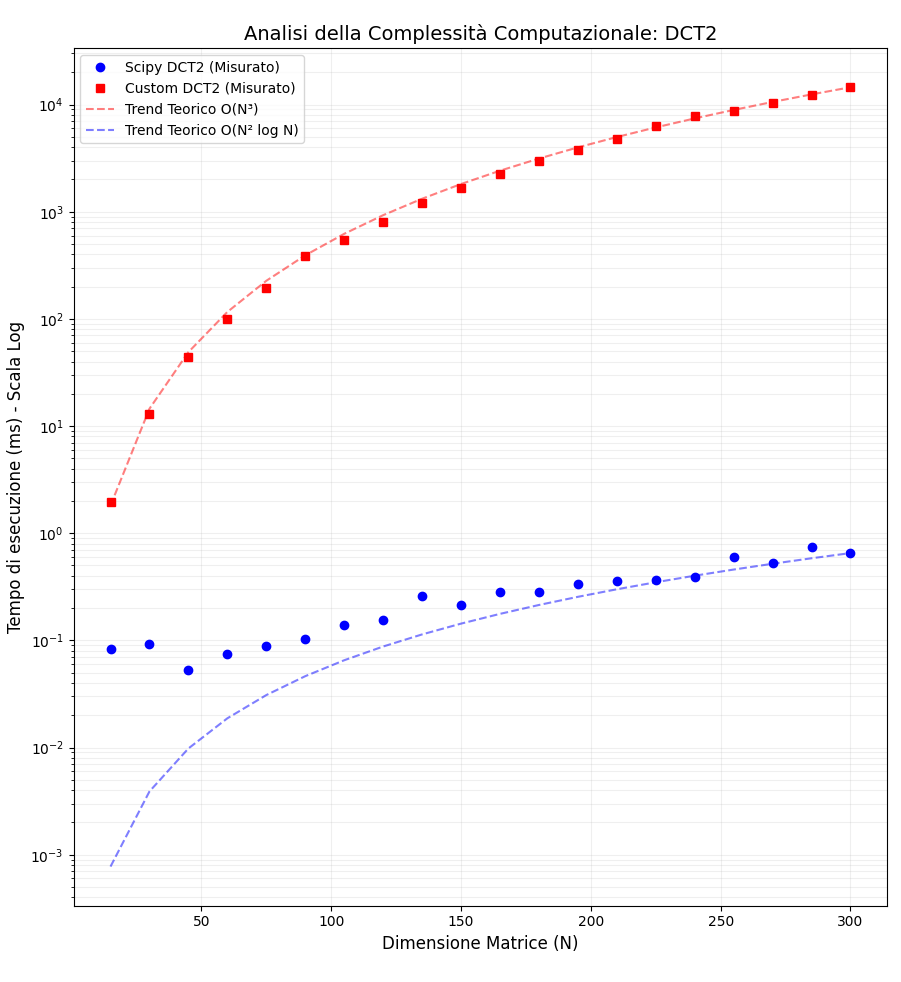
\includegraphics[width=0.75\textwidth]{images/benchmark_plot.png}
  \caption{Confronto dei tempi di esecuzione (scala semi-log) tra la DCT2
           custom ($O(N^3)$) e quella SciPy ($O(N^2 \log N)$).
           Le curve tratteggiate mostrano le tendenze teoriche normalizzate
           sull'ultimo punto misurato.}
  \label{fig:benchmark}
\end{figure}

Come atteso dalla teoria:
\begin{itemize}
  \item La DCT2 custom cresce come $O(N^3)$: per ciascuna delle $2N$ applicazioni
        della DCT monodimensionale il costo è $O(N^2)$, per un totale di
        $O(N^3)$.
  \item La DCT2 di SciPy, basata sull'algoritmo FFT, cresce come
        $O(N^2 \log N)$: per ciascuno degli $N$ vettori di lunghezza $N$
        si applica una FFT con costo $O(N \log N)$.
\end{itemize}
Già per $N \approx 50$ il divario supera un ordine di grandezza; per
$N = 200$ la versione custom è circa $10^2$--$10^3$ volte più lenta.
Si nota inoltre che l'implementazione di libreria presenta un andamento iniziale
relativamente irregolare (per $N$ molto piccoli), mentre la curva della DCT
custom segue fedelmente l'andamento $O(N^3)$ già dai primi valori.  
Nella pipeline di compressione (\texttt{jpeg.py}) viene usata la DCT2 custom
per rispettare i requisiti del progetto (SciPy è impiegata solo nel benchmark).

% ─────────────────────────────────────────────────────────────────────────────
\section{Parte II -- Software di compressione}
% ─────────────────────────────────────────────────────────────────────────────

\subsection{Struttura del progetto}

Il codice è organizzato nei seguenti moduli:

\begin{description}[leftmargin=3.5cm, style=nextline]
  \item[\texttt{utils.py}]   DCT/IDCT monodimensionali e DCT2/IDCT2 custom.
  \item[\texttt{jpeg.py}]    Suddivisione in blocchi, compressione di un singolo
                             blocco, compressione parallela su più core dell'immagine .
  \item[\texttt{gui.py}]     Interfaccia grafica (PyQt6): splash screen, pannello
                             di controllo, visualizzazione side-by-side.
  \item[\texttt{CLI.py}]     Interfaccia a riga di comando (argparse).
  \item[\texttt{main.py}]    Entry point: avvia la GUI se non vengono passati
                             argomenti, altrimenti la CLI.
  \item[\texttt{styles.py}]  Palette grafica dark e messaggi dello splash screen.
  \item[\texttt{tests.py}]   Test di correttezza della DCT/DCT2 sul blocco campione.
  \item[\texttt{benchmark.py}] Benchmark custom vs SciPy con grafico.
\end{description}

\subsection{Pipeline di compressione (\texttt{jpeg.py})}

\paragraph{Suddivisione in blocchi.}
La funzione \texttt{block\_splitter} ritaglia l'immagine alla dimensione più
vicina multiplo di $F$ (in eccesso verso il basso) e restituisce la lista dei
blocchi $F\times F$ ordinati per riga:

\begin{lstlisting}[caption={Suddivisione in blocchi -- \texttt{jpeg.py}}]
def block_splitter(A, F):
    h, w = A.shape
    n_y, n_x = h // F, w // F
    A = A[: n_y*F, : n_x*F].astype(float)
    return n_y, n_x, [
        A[by*F:(by+1)*F, bx*F:(bx+1)*F]
        for by in range(n_y)
        for bx in range(n_x)
    ]
\end{lstlisting}

\paragraph{Compressione di un blocco.}
La funzione \texttt{compress\_block} applica la DCT2, azzera i coefficienti
con $k+\ell \geq d$ tramite una maschera NumPy efficiente, e ricostruisce il
blocco con la IDCT2:

\begin{lstlisting}[caption={Compressione di un blocco -- \texttt{jpeg.py}}]
def compress_block(block, d):
    c = dct2(block)
    F = block.shape[0]
    k, l = np.meshgrid(np.arange(F), np.arange(F), indexing="ij")
    c[k + l >= d] = 0.0
    return np.clip(np.round(idct2(c)), 0, 255).astype(np.uint8)
\end{lstlisting}

\paragraph{Compressione parallela dell'immagine.}
Per ridurre i tempi di elaborazione su immagini di grandi dimensioni, la
funzione \texttt{compress\_image} distribuisce i blocchi su
$\max(1,\;\text{cpu\_count}-2)$ processi tramite
\texttt{concurrent.futures.ProcessPoolExecutor} richiamando la funzione \textbf{compress\_block} in maniera parallela su ogni blocco;
successivamente prende tutti i blocchi compressi e ricostruisce l'immagine:

\begin{lstlisting}[caption={Compressione parallela dell'immagine -- \texttt{jpeg.py}}]
def compress_image(img, F, d):
    A = np.array(img.convert("L"))
    n_y, n_x, blocks = block_splitter(A, F)
    max_cores = max(1, (os.cpu_count() or 1) - 2)
    with ProcessPoolExecutor(max_workers=max_cores) as executor:
        compressed = list(executor.map(compress_block,
                                       blocks, [d]*len(blocks)))
    rows = [np.hstack(compressed[by*n_x:(by+1)*n_x]) for by in range(n_y)]
    return Image.fromarray(np.vstack(rows))
\end{lstlisting}

\paragraph{Validazione dei parametri.}
La funzione \texttt{validate\_params} controlla che $F \geq 1$,
$F \leq \min(\text{larghezza},\, \text{altezza})$ e
$d \in [0,\, 2F-2]$, restituendo un messaggio di errore descrittivo in caso
di violazione.

\subsection{Interfaccia Grafica (GUI)}

L'interfaccia grafica è realizzata con \textbf{PyQt6} e adotta una palette
dark ispirata al tema Catppuccin Mocha. La finestra è organizzata in:
\begin{itemize}
  \item \textbf{Header}: logo dell'università (opzionale), titolo e autori.
  \item \textbf{Barra di controllo}: percorso file (con bottone \emph{Browse}),
        campi $F$ e $d$, bottone \emph{Process}.
  \item \textbf{Area immagini}: due pannelli affiancati per l'originale e la
        compressa, ridimensionabili dinamicamente.
  \item \textbf{Status bar}: messaggi di stato sull'avanzamento.
\end{itemize}
In pratica, la parte superiore della finestra contiene i controlli per la
selezione dell'immagine e l'impostazione dei parametri, mentre la parte
inferiore è suddivisa in due pannelli che mostrano fianco a fianco
l'immagine originale e quella compressa.

L'elaborazione avviene in un thread separato (\texttt{ProcessorThread},
sottoclasse di \texttt{QThread}) per non bloccare l'interfaccia durante la
compressione. I tasti \texttt{Return}/\texttt{Enter} sono collegati tramite
\texttt{QShortcut} al bottone \emph{Process}.

All'avvio viene mostrato uno \textbf{splash screen} animato con una sequenza
di messaggi umoristici, realizzato con \texttt{QSplashScreen} e un pixmap
generato programmaticamente.

\begin{figure}[H]
  \centering
  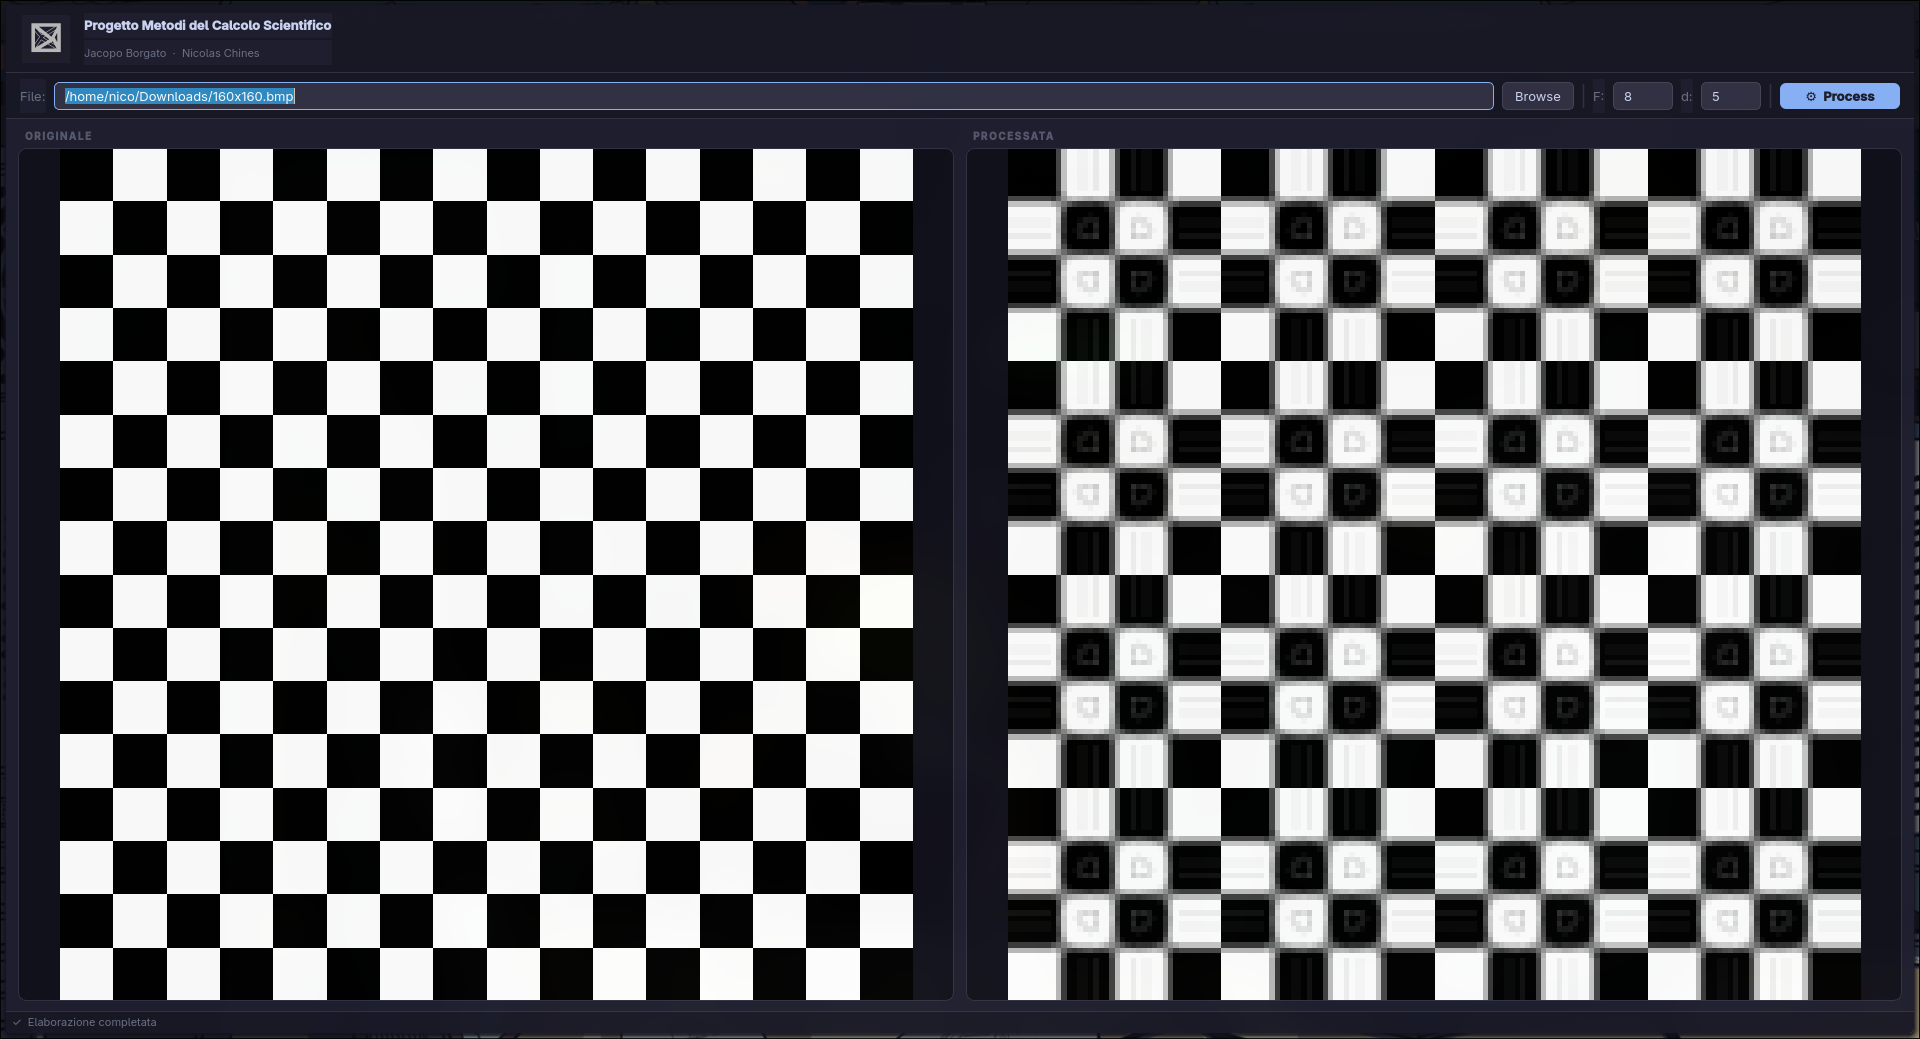
\includegraphics[width=0.88\textwidth]{images/gui_screenshot.png}
  \caption{Interfaccia grafica: a sinistra l'immagine originale, a destra quella
           compressa con $F=8$, $d=5$.}
  \label{fig:gui}
\end{figure}

\subsection{Interfaccia a riga di comando (CLI)}

La CLI (\texttt{CLI.py}) utilizza \texttt{argparse} e accetta i seguenti
argomenti:

\begin{lstlisting}[language=bash, caption={Sintassi CLI}]
python main.py <immagine.bmp> <F> <d> [-o output.bmp] [-s]
\end{lstlisting}

L'opzione \texttt{-o}/\texttt{--output} salva l'immagine compressa su disco;
\texttt{-s}/\texttt{--show} visualizza le due immagini affiancate.
Al termine viene stampato un riepilogo con le dimensioni, i parametri scelti
e la percentuale di coefficienti mantenuti per blocco.

Esempio:
\begin{lstlisting}[language=bash]
python main.py photo.bmp 8 5 --output result.bmp --show
# Output:
# Image   : photo.bmp  (512 x 512 px)
# F = 8,  d = 5
# Kept    : 15 / 64 coefficients per block  (23 %)
# Output  : 512 x 512 px  (cropped to multiple of F)
# Saved   : result.bmp
\end{lstlisting}

% ─────────────────────────────────────────────────────────────────────────────
\section{Risultati sperimentali}
% ─────────────────────────────────────────────────────────────────────────────

\subsection{Effetto del parametro $d$}

Per analizzare l’effetto del parametro $d$, è stata fissata la dimensione
del blocco a $F = 20$ ed è stato variato il numero di coefficienti mantenuti
nella trasformata DCT.

\subsubsection*{Caso $d = 0$}

Tutti i coefficienti DCT vengono annullati.  
L’immagine ricostruita risulta completamente nera, poiché ogni blocco assume
valore nullo.

\begin{figure}[H]
    \centering
    
\includegraphics[width=0.38\textwidth,keepaspectratio]{images/shoe_F20_d0.png}
    \caption{Compressione con $F=20$, $d=0$.}
\end{figure}

\subsubsection*{Caso $d = 1$}

Viene mantenuto solamente il coefficiente DC
(corrispondente alla media del blocco).  
Ogni blocco assume quindi un colore uniforme e l’immagine appare fortemente
pixelata, con perdita quasi totale dei dettagli.

\begin{figure}[H]
    \centering
    
\includegraphics[width=0.38\textwidth,keepaspectratio]{images/shoe_F20_d1.png}
    \caption{Compressione con $F=20$, $d=1$.}
\end{figure}

\subsubsection*{Caso $d = 15$}

Si conservano le componenti a bassa e media frequenza.  
La struttura generale dell’immagine rimane riconoscibile, ma i bordi risultano
più sfumati e iniziano a comparire artefatti dovuti alla suddivisione in blocchi.

\begin{figure}[H]
    \centering
    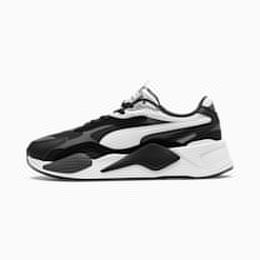
\includegraphics[width=0.38\textwidth,keepaspectratio]{images/shoe_F20_d15.png}
    \caption{Compressione con $F=20$, $d=15$.}
\end{figure}

\subsubsection*{Caso $d = 38$}

Questo valore rappresenta il massimo consentito
($d = 2F - 2 = 38$ per $F=20$).  
Viene eliminata solamente la componente di frequenza più alta; la differenza
rispetto all’immagine originale risulta praticamente impercettibile.

\begin{figure}[H]
    \centering
    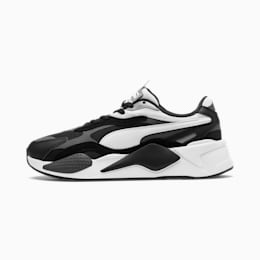
\includegraphics[width=0.38\textwidth,keepaspectratio]{images/shoe_F20_d38.png}
    \caption{Compressione con $F=20$, $d=38$.}
\end{figure}

% ─────────────────────────────────────────────────────────────────────────────

\subsection{Effetto del parametro $F$}

Per studiare l’influenza della dimensione dei blocchi, è stato fissato
$d = 2$ e sono stati confrontati diversi valori di $F$.

\subsubsection*{Caso $F = 4$, $d = 2$}

Con blocchi piccoli gli artefatti sono meno evidenti e l’immagine appare
più uniforme. Tuttavia, la capacità di compressione è limitata.

\begin{figure}[H]
    \centering
    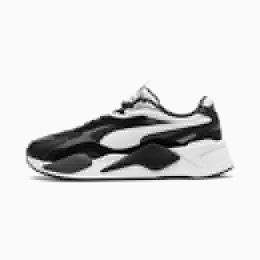
\includegraphics[width=0.38\textwidth,keepaspectratio]{images/shoe_F4_d2.png}
    \caption{Compressione con $F=4$, $d=2$.}
\end{figure}

\subsubsection*{Caso $F = 16$, $d = 2$}

Aumentando la dimensione dei blocchi, la compressione diventa più aggressiva.
La struttura a blocchi inizia a essere visibile e alcuni dettagli fini vengono persi.

\begin{figure}[H]
    \centering
    
\includegraphics[width=0.38\textwidth,keepaspectratio]{images/shoe_F16_d2.png}
    \caption{Compressione con $F=16$, $d=2$.}
\end{figure}

\subsubsection*{Caso $F = 32$, $d = 2$}

Con blocchi molto grandi gli artefatti diventano fortemente evidenti.
L’immagine presenta aree uniformi estese e una marcata perdita di dettaglio,
pur ottenendo una compressione più elevata.

\begin{figure}[H]
    \centering
    
\includegraphics[width=0.38\textwidth,keepaspectratio]{images/shoe_F32_d2.png}
    \caption{Compressione con $F=32$, $d=2$.}
\end{figure}

\subsection{Tabella riassuntiva}

La Tabella~\ref{tab:results} riporta il numero di coefficienti mantenuti per
blocco nei test effettuati, insieme alla percentuale rispetto al totale dei
coefficienti disponibili ($F^2$).

\begin{table}[H]
\centering
\caption{Coefficienti mantenuti per blocco nei test sperimentali.}
\label{tab:results}
\begin{tabular}{ccccc}
\toprule
$F$ & $d$ & Coefficienti mantenuti & Totale ($F^2$) & Percentuale \\
\midrule
20 & 0  &   0   & 400  &   0\% \\
20 & 1  &   1   & 400  &   0.25\% \\
20 & 15 & 120   & 400  &  30\% \\
20 & 38 & 399   & 400  &  99.75\% \\
\midrule
4  & 2  &   3   & 16   &  18.75\% \\
16 & 2  &   3   & 256  &  1.17\% \\
32 & 2  &   3   & 1024 &  0.29\% \\
\bottomrule
\end{tabular}
\end{table}

% ── Nuovi test aggiuntivi (dal secondo documento) ─────────────────────────
\subsection{Test aggiuntivi}
\label{sec:test_aggiuntivi}

Per evidenziare il comportamento dell'algoritmo in situazioni limite sono stati
condotti ulteriori esperimenti: una verifica con immagini composte da quadrati
regolari e l'osservazione del fenomeno di Gibbs.

\subsubsection{Suddivisione in quadrati regolari}

Si è utilizzata un'immagine sintetica contenente quadrati uniformi di lato noto,
in modo da valutare l'allineamento tra i blocchi di compressione e la geometria
dell'immagine. Le Figure~\ref{fig:perfect_subdivision}, \ref{fig:11x_squares} e
\ref{fig:15x_squares} mostrano il risultato della compressione con $d=1$
(solo il coefficiente DC) per dimensioni del macro-blocco $F = 10$, $11$ e $15$,
rispettivamente.

\begin{figure}[H]
	\centering
	\begin{subfigure}[b]{0.3\textwidth}
		\centering
		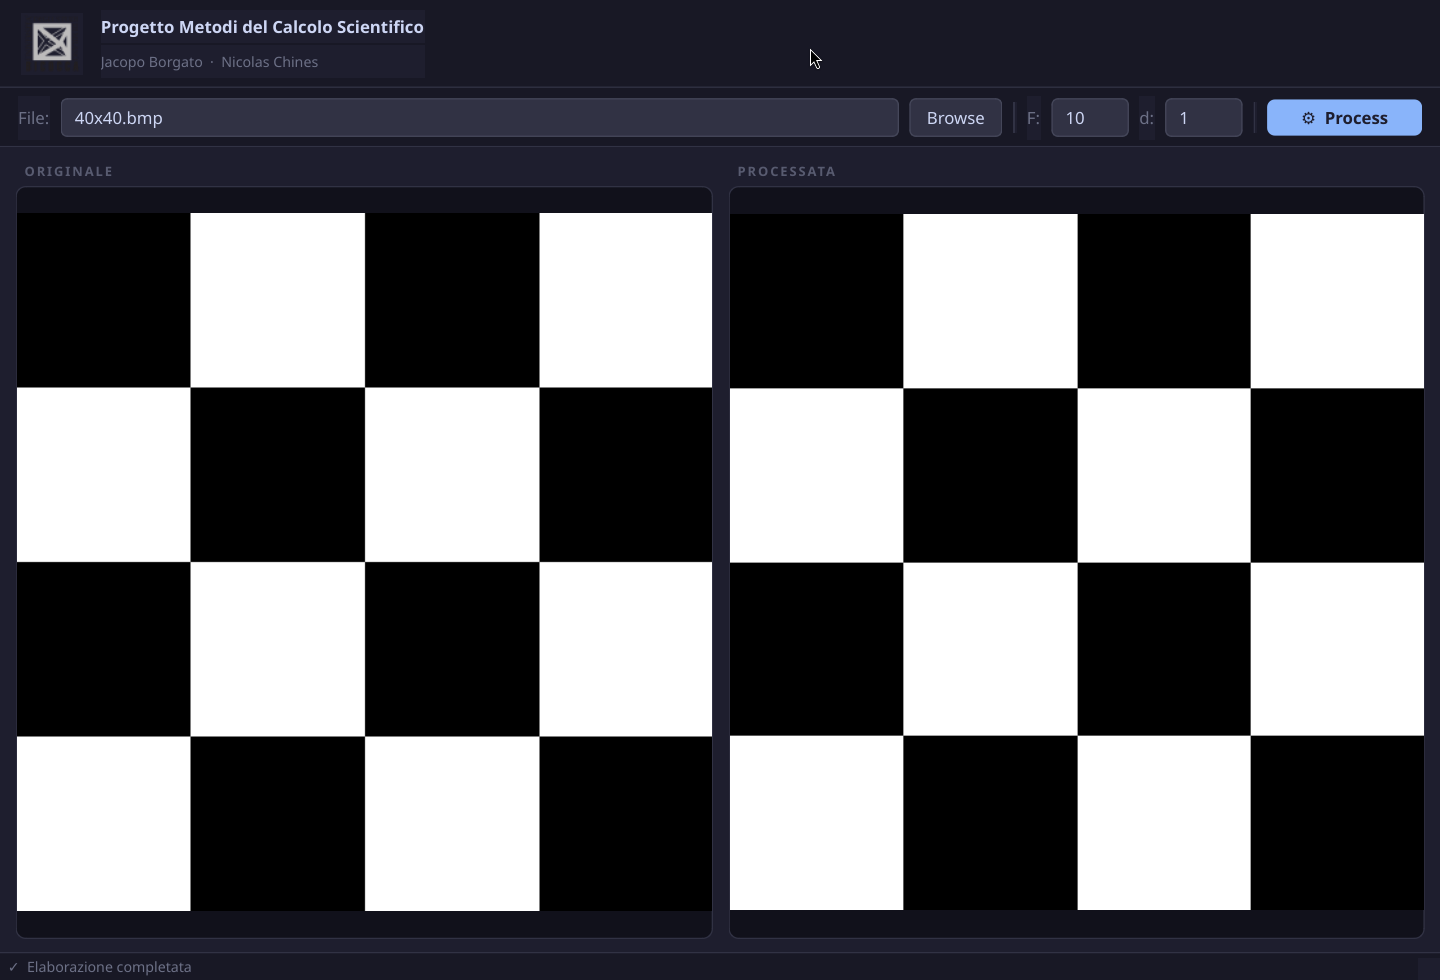
\includegraphics[width=\textwidth]{images/perfect_squares.png}
		\caption{$F=10$ .}
		\label{fig:perfect_subdivision}
	\end{subfigure}
	\hfill
	\begin{subfigure}[b]{0.3\textwidth}
		\centering
		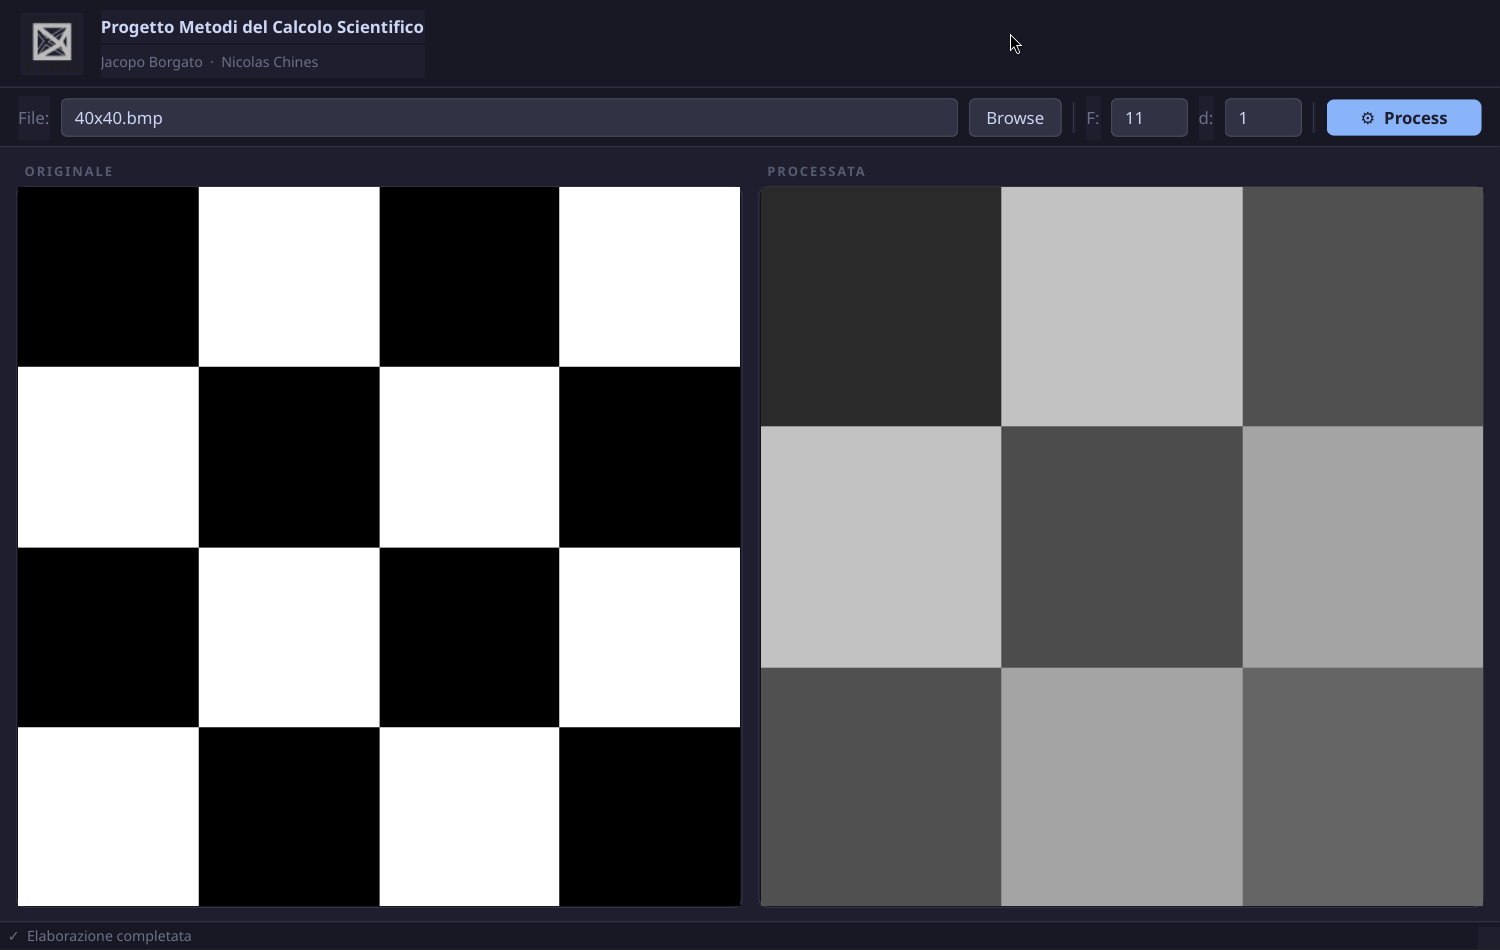
\includegraphics[width=\textwidth]{images/11x_squares.png}
		\caption{$F=11$ .}
		\label{fig:11x_squares}
	\end{subfigure}
	\hfill
	\begin{subfigure}[b]{0.3\textwidth}
		\centering
		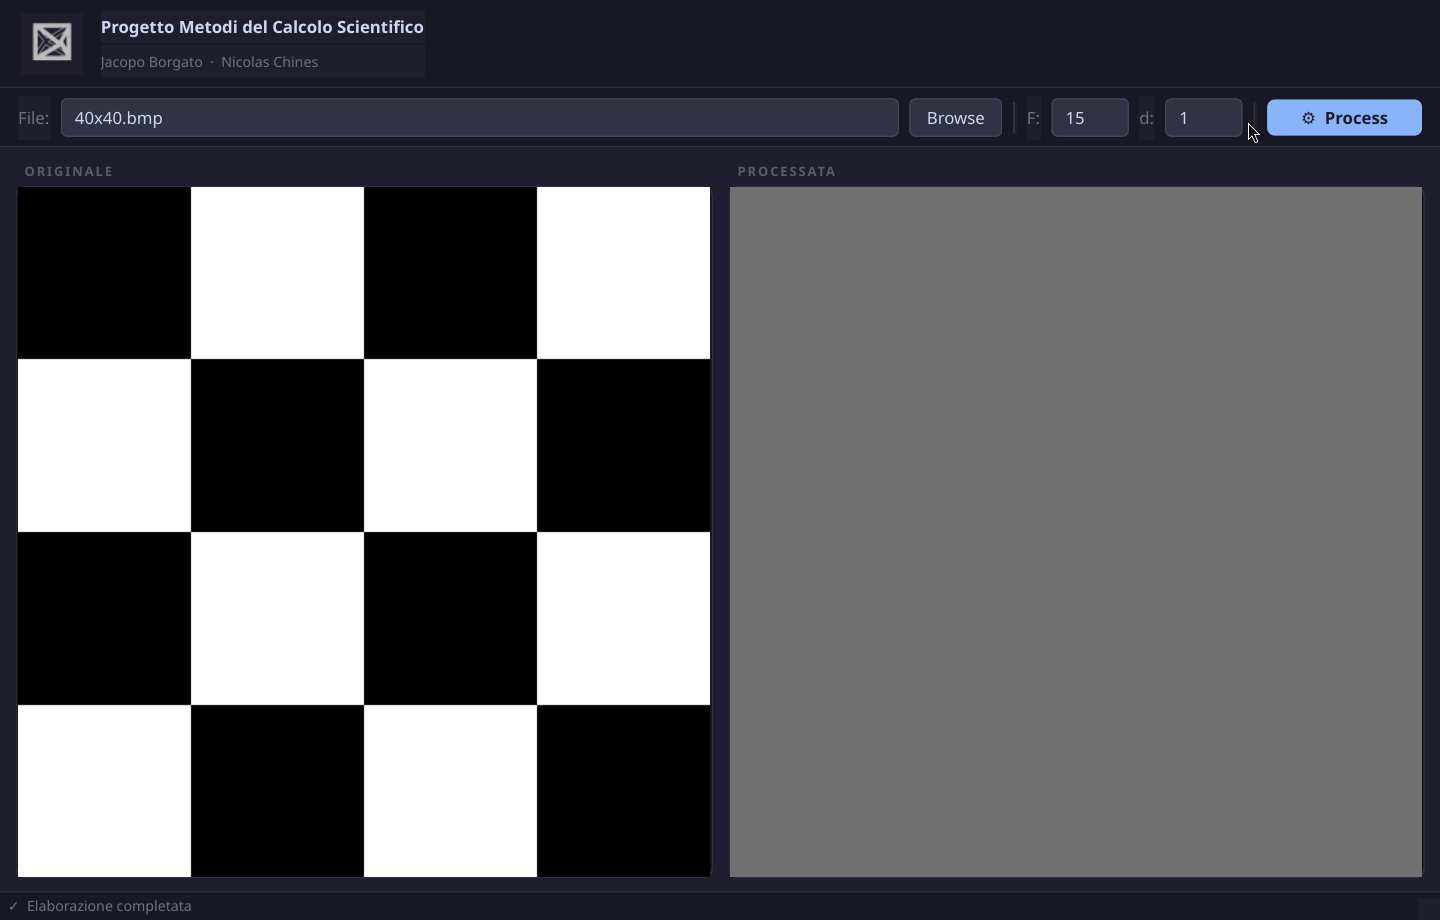
\includegraphics[width=\textwidth]{images/15x_squares.png}
		\caption{$F=15$.}
		\label{fig:15x_squares}
	\end{subfigure}
	\caption{Effetto della dimensione del blocco su un'immagine a quadrati
	         uniformi ($d=1$).}
	\label{fig:squares_images}
\end{figure}

Quando $F$ è un multiplo esatto della dimensione dei quadrati (Fig.~\ref{fig:perfect_subdivision}),
la suddivisione in blocchi coincide perfettamente con la struttura dell’immagine.
Poiché nel caso $d=1$ viene mantenuto esclusivamente il coefficiente DC (cioè la media del blocco),
ogni blocco di compressione assume esattamente il colore medio del quadrato originale.
Essendo l’immagine una scacchiera di regioni uniformi, la media coincide con il valore stesso del quadrato,
e la ricostruzione risulta praticamente identica all’originale.

Nel caso $F=11$ (Fig.~\ref{fig:11x_squares}), la dimensione dei blocchi non è più allineata
con la struttura geometrica dell’immagine. I blocchi attraversano i bordi dei quadrati,
mescolando pixel appartenenti a regioni con intensità diverse: di conseguenza la media interna
non corrisponde più a un singolo colore uniforme, ma a una combinazione dei due. Questo produce
artefatti evidenti lungo i bordi, che appaiono come transizioni in scala di grigi tra i quadrati.
Inoltre, l’eliminazione delle alte frequenze ($d=1$) impedisce la rappresentazione di tali discontinuità,
accentuando l’effetto di sfumatura lungo le diagonali e i bordi dei blocchi.

Infine, con $F=15$ (Fig.~\ref{fig:15x_squares}) la dimensione dei blocchi diventa molto più grande
rispetto alla struttura dell’immagine. Ogni blocco contiene porzioni di più quadrati e quindi la media
risultante tende a uniformare ulteriormente l’intensità locale. Poiché viene mantenuto solo il termine DC,
la ricostruzione perde completamente le variazioni spaziali interne, producendo un’immagine quasi uniforme
in tonalità di grigio. Questo spiega la forte perdita di dettaglio e l’aspetto “appiattito” del risultato.

\subsubsection{Fenomeno di Gibbs}

La troncatura dei coefficienti DCT ad alta frequenza introduce oscillazioni
note come \emph{fenomeno di Gibbs}, particolarmente visibili in prossimità di
bordi netti. La Figura~\ref{fig:gibbs} mostra un esempio su un'immagine con
una transizione brusca; l'ingrandimento in Figura~\ref{fig:gibbs_zoom}
evidenzia le oscillazioni (ringing) attorno al bordo.

\begin{figure}[H]
	\centering
	\begin{subfigure}[b]{0.5\textwidth}
		\centering
		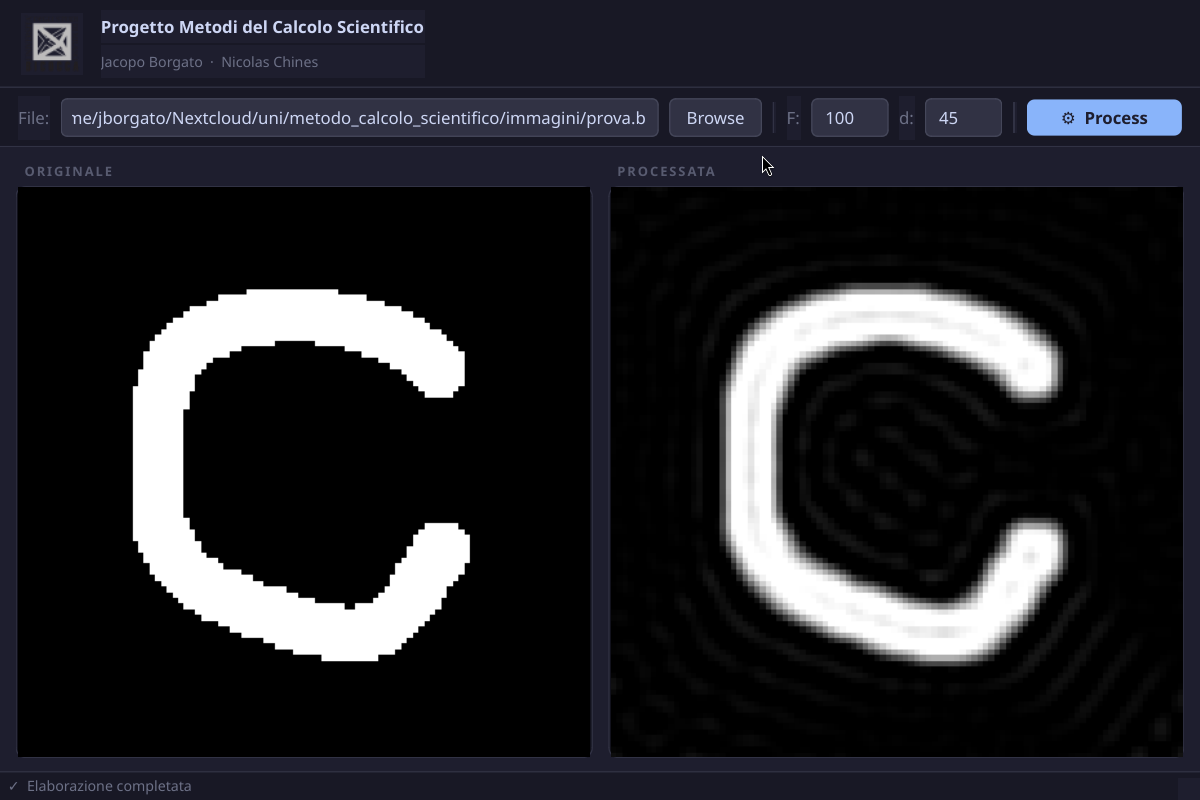
\includegraphics[width=\textwidth]{images/gibbs.png}
		\caption{Immagine compressa con $F=8$, $d=4$.}
		\label{fig:gibbs}
	\end{subfigure}
	\hfill
	\begin{subfigure}[b]{0.37\textwidth}
		\centering
		
\includegraphics[width=\textwidth]{images/gibbs_zoom.png}
		\caption{Dettaglio del ringing attorno al bordo.}
		\label{fig:gibbs_zoom}
	\end{subfigure}
	\caption{Fenomeno di Gibbs dovuto alla soppressione delle alte frequenze.}
	\label{fig:gibbs_graphs}
\end{figure}

Questi artefatti sono intrinseci al metodo di compressione e diventano più
evidenti quando vengono mantenuti pochi coefficienti ($d$ piccolo). Riducendo
la dimensione del blocco $F$ l'effetto si manifesta su scale spaziali più
piccole, risultando meno percepibile globalmente.

% ─────────────────────────────────────────────────────────────────────────────
\section{Considerazioni sull'aritmetica in virgola mobile}
% ─────────────────────────────────────────────────────────────────────────────

Tutti i calcoli sono eseguiti in doppia precisione (\texttt{float64}), con
machine epsilon $\varepsilon_{\text{mach}} = 2^{-52} \approx 2.22\times 10^{-16}$.

Il passo di arrotondamento e clipping finale (\texttt{np.clip(np.round(...), 0, 255)})
è essenziale: senza di esso, piccoli errori numerici accumulati durante la
IDCT2 possono produrre valori leggermente fuori dall'intervallo $[0, 255]$
o valori frazionari non rappresentabili come pixel a 8 bit.
In pratica tali errori sono dell'ordine di $10^{-10}$--$10^{-12}$,
ampiamente al di sotto della soglia di un'unità su 255.

% ─────────────────────────────────────────────────────────────────────────────
\section{Conclusioni}
% ─────────────────────────────────────────────────────────────────────────────

Il progetto ha permesso di implementare e verificare un algoritmo di
compressione di immagini JPEG-like completo:

\begin{itemize}
  \item La DCT2 custom è stata validata sul blocco campione fornito dal
        docente, ottenendo risultati conformi ai valori attesi.
  \item Il benchmark ha confermato le complessità teoriche $O(N^3)$ per la
        versione custom e $O(N^2 \log N)$ per SciPy, evidenziando l'importanza
        degli algoritmi FFT per applicazioni su larga scala.
  \item L'interfaccia grafica PyQt6 e la CLI consentono un utilizzo flessibile
        del software; il parallelismo via \texttt{ProcessPoolExecutor} riduce
        sensibilmente i tempi su macchine multi-core.
  \item Gli esperimenti mostrano un chiaro \emph{trade-off} tra qualità visiva
        e compressione al variare di $d$: valori bassi producono immagini
        degradate ma altamente compresse, mentre valori alti preservano quasi
        interamente la qualità originale.
  \item I test aggiuntivi sulla suddivisione in quadrati e sul fenomeno di Gibbs
        confermano che l'allineamento dei blocchi e la troncatura delle
        frequenze influenzano in modo determinante la percezione degli artefatti.
\end{itemize}

La principale limitazione dell'implementazione corrente è l'uso della DCT2
custom (lenta) nella pipeline di compressione anziché di quella SciPy.
Un'estensione naturale sarebbe sostituirla con \texttt{scipy.fftpack.dctn}
per rendere il software fruibile su immagini ad alta risoluzione.

% ─────────────────────────────────────────────────────────────────────────────
\appendix
\section{Istruzioni per l'esecuzione}
% ─────────────────────────────────────────────────────────────────────────────

\subsection{Requisiti}

\begin{lstlisting}[language=bash]
pip install numpy scipy pillow pyqt6 matplotlib
\end{lstlisting}

\subsection{Avvio dell'interfaccia grafica}

\begin{lstlisting}[language=bash]
python main.py
\end{lstlisting}

\subsection{Utilizzo da riga di comando}

\begin{lstlisting}[language=bash]
python main.py <immagine.bmp> <F> <d>
python main.py immagine.bmp 8 5 --output compressa.bmp --show
python main.py immagine.bmp 8 0   # immagine completamente bianca
\end{lstlisting}

\subsection{Test di correttezza}

\begin{lstlisting}[language=bash]
python tests.py
# Testing on Array: True
# Testing on Matrix: True
\end{lstlisting}

\subsection{Benchmark}

\begin{lstlisting}[language=bash]
python benchmark.py
\end{lstlisting}

\end{document}